\section{The Dot Product} \label{S:9.3.Dot_Product}

\vspace*{-14 pt}
\framebox{\hspace*{3 pt}
\parbox{6.25 in}{\begin{goals}
  \item How is the dot product of two vectors defined and what
    geometric information does it tell us? 
  \item How can we tell if two vectors in $\R^n$ are perpendicular?
  \item How do we find the projection of one vector onto another?
\end{goals}} \hspace*{3 pt}}

\subsection*{Introduction}

In the last section, we considered vector addition and scalar
multiplication and found that each operation had a natural geometric
interpretation.  In this section, we will introduce a means of
multiplying vectors.

\begin{pa} \label{PA:9.3}
  For two-dimensional vectors $\vu=\langle u_1,u_2\rangle$ and
  $\vv=\langle v_1, v_2\rangle$, the dot product is simply the scalar
  obtained by
  $$
  \vu\cdot\vv = u_1v_1 + u_2v_2.
  $$

    \ba
  \item If $\vu=\langle 3, 4\rangle$ and $\vv=\langle -2, 1\rangle$,
    find the dot product $\vu\cdot\vv$.

  \item Find $\vi\cdot\vi$ and $\vi\cdot\vj$.

  \item If $\vu=\langle 3, 4\rangle$, find $\vu\cdot\vu$.  How is this
    related to $|\vu|$?

  \item On the axes in Figure \ref{F:9.3.preview.1}, plot the
    vectors $\vu=\langle 1, 3\rangle$ and $\vv=\langle -3, 1\rangle$.  Then, 
    find $\vu\cdot\vv$.  What is the angle between these vectors?  

    \begin{figure}[ht]
      \begin{center}
        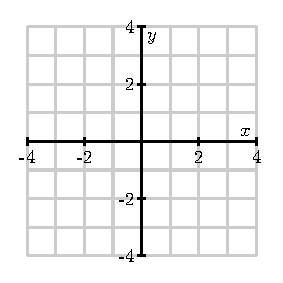
\includegraphics{figures/fig_9_3_preview_1.eps}
        \caption{For part (d)}
        \label{F:9.3.preview.1}
      \end{center}
    \end{figure}

  \item On the axes in Figure \ref{F:9.3.preview.2}, plot the
    vector $\vu=\langle 1, 3\rangle$.

    \begin{figure}[ht]
      \begin{center}
        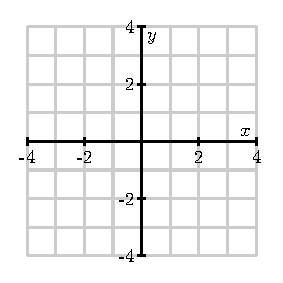
\includegraphics{figures/fig_9_3_preview_1.eps}
        \caption{For part (e)}
        \label{F:9.3.preview.2}
      \end{center}
    \end{figure}

    For each of the following vectors $\vv$, plot the vector on Figure
    \ref{F:9.3.preview.2} and then compute the dot product
    $\vu\cdot\vv$. 

    \begin{itemize}
      \item $\vv=\langle 3, 2 \rangle$.
      \item $\vv=\langle 3, 0 \rangle$.
      \item $\vv=\langle 3,-1 \rangle$.
      \item $\vv=\langle 3,-2 \rangle$.
      \item $\vv=\langle 3,-4 \rangle$.
      \end{itemize}

    \item Based upon the previous part of this activity, what do you
      think is the sign of the dot product in the following three
      cases shown in Figure \ref{F:9.3.preview.3}?

    \begin{figure}[ht]
      \begin{center}
        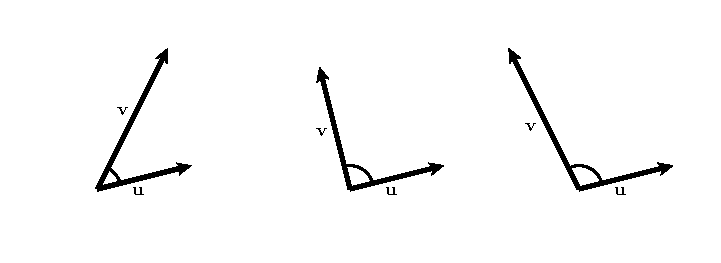
\includegraphics{figures/fig_9_3_preview_2.eps}
        \caption{For part (f)}
        \label{F:9.3.preview.3}
      \end{center}
    \end{figure}

      


    \ea

\end{pa} 

\begin{activitySolution}
    \ba
  \item Here we have $u_1=3$, $u_2=4$, $v_1=-2$, and $v_2=1$, so 
\[\vu \cdot \vv = \langle 3, 4\rangle \cdot \langle -2, 1\rangle = (3)(-2)+(4)(1) = -2.\]

  \item Since $\vi = \langle 1,0 \rangle$ and $\vj = \langle 0,1 \rangle$, it follows that 
\[\vi\cdot\vi = 1 \ \text{ and } \ \vi\cdot\vj = 0.\]

  \item In this case we have 
\[\vu \cdot \vu = \langle 3, 4\rangle \cdot \langle 3, 4\rangle = 3^2+4^2 = 25.\]
By the distance formula, the length of $\vu$ is 
\[|\vu| = \sqrt{3^2+4^2} = 5.\]
So $\vu \cdot \vu = |\vu|^2$. 

  \item The slope of the line through the origin and the point $(1,3)$ is 1 while the slope of the line through the origin and the point $(-3,1)$ is $-\frac{1}{3}$. Since these slopes are negative reciprocals, the lines are perpendicular. Thus, the angle between $\vu$ and $\vv$ is $90^{\circ}$. Also
\[\vu \cdot \vv = \langle 1, 3\rangle \cdot \langle -3, 1\rangle = (1)(-3)+(3)(1) = 0.\]

  \item With $\vu=\langle 1, 3\rangle$ we have 
    \begin{itemize}
      \item $\vu \cdot \langle 3, 2 \rangle = \langle 1, 3\rangle \cdot \langle 3, 2 \rangle = 9$.
      \item $\vu \cdot \langle 3, 0 \rangle = \langle 1, 3\rangle \cdot \langle 3, 0 \rangle = 1$.
      \item $\vu \cdot \langle 3, -1 \rangle = \langle 1, 3\rangle \cdot \langle 3, -1 \rangle = 0$.
      \item $\vu \cdot \langle 3, -4 \rangle = \langle 1, 3\rangle \cdot \langle 3, -4 \rangle = -9$.
      \end{itemize}

    \item If two vectors are perpendicular, it appears that their dot product is 0. If the vectors form an acute angle (less than $90^{\circ}$ as with $\vu$ and $\langle 3,2 \rangle$ or $\langle 3,0 \rangle$ from the previous part of this activity), then it looks as though their dot product is positive. Finally, if the vectors form an obtuse (greater than $90^{\circ}$ as with $\vu$ and $\langle 3,-4 \rangle$ from the previous part of this activity), then it looks as though their dot product is negative. 
    \ea
\end{activitySolution}

\afterpa 

\subsection*{The Dot Product}

If we have two $n$-dimensional vectors 
$\vu=\langle u_1, u_2,\ldots,u_n\rangle$ 
and 
$\vv=\langle v_1, v_2,\ldots,v_n\rangle$, we define their \emph{dot
product}\footnote{As we will see shortly, the dot product arises in physics to calculate the work done by a vector force in a given direction. It might be more natural to define the dot product in this context, but it is more convenient from a mathematical perspective to define the dot product algebraically and then view work as an application of this definition.}\index{dot product} as
$$
\vu\cdot\vv = u_1v_1+u_2v_2 + \ldots + u_nv_n.
$$
For instance, we find that
$$
\langle 3, 0, 1 \rangle\cdot\langle -2, 1, 4\rangle = 3\cdot(-2) +
0\cdot1 + 1\cdot4 = -6 + 0 + 4 = -2.
$$
Notice that the resulting quantity is a scalar.  Our work in Preview
Activity \ref{PA:9.3} examined dot products of two-dimensional
vectors.  

\begin{activity} \label{A:9.3.2}  Determine each of the following.
  \ba
\item $\langle 1, 2, -3 \rangle \cdot \langle 4, -2, 0 \rangle$.

\item $\langle 0, 3, -2, 1 \rangle \cdot \langle 5, -6, 0, 4 \rangle$

  \ea
\end{activity}

\begin{activitySolution}
	\ba
	\item By definition $\langle 1, 2, -3 \rangle \cdot \langle 4, -2, 0 \rangle = 0$.
	
	\item By definition $\langle 0, 3, -2, 1 \rangle \cdot \langle 5, -6, 0, 4 \rangle = -14$.
	\ea
\end{activitySolution}

\aftera



The dot product is a natural way to define a product of two vectors.
In addition, it behaves in ways that are similar to the product of,
say, real numbers.

\vspace*{5pt}
\nin 
\framebox{\hspace*{3 pt}
  \parbox{6.25 in}{
    Let $\vu$, $\vv$, and $\vw$ be vectors in $\R^n$. Then
    \ba
  \item $\vu \cdot \vv = \vv \cdot \vu$ (the dot product is
    \emph{commutative}), and
  \item if $c$ is a scalar, then $(c\vu + \vv) \cdot \vw = c(\vu \cdot
    \vw) + \vv \cdot \vw$ (the dot product is \emph{bilinear}),
    \ea
  } \hspace*{3 pt}}
\vspace*{5pt}

Moreover, the dot product gives us valuable geometric information
about the vectors and their relative orientation.  For instance, let's
consider what happens when we dot a vector with itself:
$$
\vu\cdot\vu = \langle u_1,u_2,\ldots,u_n \rangle \cdot \langle u_1,u_2,\ldots,u_n \rangle = 
u_1^2 + u_2^2 + \ldots + u_n^2 = |\vu|^2.
$$
In other words, the dot product of a vector with itself gives the
square of the length of the vector:  $\vu\cdot\vu=|\vu|^2$.  

\subsection*{The angle between vectors}

The dot product can help us understand the angle between two
vectors.  For instance, if we are given two vectors $\vu$ and $\vv$,
there are two angles that these vectors create, as depicted in Figure
\ref{F:9.3.Angle_between}. We will call $\theta$, the smaller of these
angles, the \emph{angle between these vectors}\index{vector!angle between}.  Notice that
$\theta$ lies between 0 and $\pi$.


\begin{figure}[ht]
  \begin{center}
    \begin{minipage}{3in}
  \begin{center}
    \scalebox{1.0}{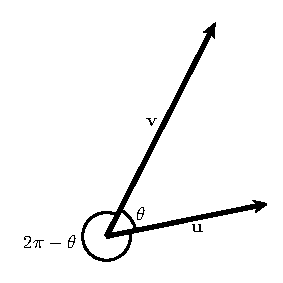
\includegraphics{figures/fig_9_3_angle_1.eps}}
    \caption{The angle between vectors $\vu$ \\ and $\vv$.}
    \label{F:9.3.Angle_between}  
  \end{center}
    \end{minipage}
    \begin{minipage}{3in}
      \begin{center}
    \scalebox{1.0}{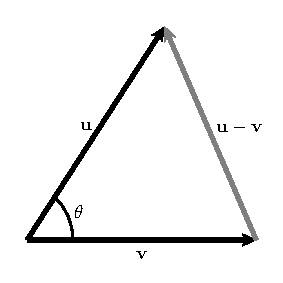
\includegraphics{figures/fig_9_3_angle_2.eps}}
    \caption{The triangle formed by $\vu$, $\vv$, and $\vu - \vv$.}
    \label{F:9.3.Angle}
  \end{center}
    \end{minipage}
  \end{center}
\end{figure}

To determine this angle, we may apply the Law of Cosines to the
triangle shown in Figure \ref{F:9.3.Angle}.  

Using the fact that the dot product of a vector with itself gives us
the square of its length, together with the bilinearity of the dot product, we find:
\begin{eqnarray*}
  |\vu-\vv|^2 & = & |\vu|^2 + |\vv|^2 - 2|\vu||\vv|\cos\theta \\
  (\vu-\vv)\cdot(\vu-\vv) &=&
  \vu\cdot\vu + \vv\cdot\vv - 2|\vu||\vv|\cos\theta \\
  \vu\cdot(\vu-\vv) - \vv\cdot(\vu-\vv)& = &
  \vu\cdot\vu + \vv\cdot\vv - 2|\vu||\vv|\cos\theta \\
  \vu\cdot\vu - 2\vu\cdot\vv + \vv\cdot\vv & = & 
  \vu\cdot\vu + \vv\cdot\vv - 2|\vu||\vv|\cos\theta \\
  -2\vu\cdot\vv & = & -2|\vu||\vv|\cos\theta \\
  \vu\cdot\vv & = & |\vu||\vv|\cos\theta.
\end{eqnarray*}
To summarize, we have the important relationship
\begin{equation}
  \vu\cdot\vv = u_1v_1+u_2v_2 + \ldots + u_nv_n =
  |\vu||\vv|\cos\theta.
  \label{E:9.3.dot.angle}
\end{equation}

It is sometimes useful to think of Equation~\eqref{E:9.3.dot.angle} as giving us an expression for
the angle between two vectors:
$$
\theta = \cos^{-1}\left(\frac{\vu\cdot\vv}{|\vu||\vv|}\right).
$$
The real beauty of this expression is this:  the dot product is a very
simple algebraic operation to perform yet it provides us with
important geometric information -- namely the angle between the vectors --
that would be difficult to determine otherwise.

\begin{activity} \label{A:9.3.2.a}  Determine each of the following.
  \ba
  \item The length of the vector $\vu=\langle 1,2,-3\rangle$ using the
    dot product.  
\item The angle between the vectors $\vu =\langle 1, 2 \rangle$ and
  $\vv = \langle 4, -1 \rangle$ to the nearest tenth of a degree. 

\item The angle between the vectors $\vy =\langle 1, 2, -3 \rangle$
  and $\vz = \langle -2, 1, 1 \rangle$ to the nearest tenth of a
  degree. 

\item If the angle between the vectors $\vu$ and $\vv$ is a right
  angle, what does the expression $\vu\cdot\vv=|\vu||\vv|\cos\theta$
  say about their dot product?

\item If the angle between the vectors $\vu$ and $\vv$ is acute---that
  is, less than $\pi/2$---what does the
  expression $\vu\cdot\vv=|\vu||\vv|\cos\theta$ say about their dot
  product?

\item If the angle between the vectors $\vu$ and $\vv$ is
  obtuse---that is, greater than $\pi/2$---what does the expression
  $\vu\cdot\vv=|\vu||\vv|\cos\theta$ say about their dot product?

  \ea
\end{activity}

\begin{activitySolution}
	\ba
	\item Since $|\vu| = \sqrt{\vu \cdot \vu}$, we have 
\[|\langle 1,2,-3\rangle| = \sqrt{1^2+2^2+(-3)^2} = \sqrt{14}.\]
	
	\item The angle $\theta$ between $\vu$ and $\vv$ is 
\[\theta = \cos^{-1}\left(\frac{\vu\cdot\vv}{|\vu||\vv|}\right) = \cos^{-1}\left(\frac{2}{\sqrt{5}\sqrt{17}}\right) \approx 77.5^{\circ}.\]

	\item The angle $\theta$ between $\vy$ and $\vz$ is 
\[\theta = \cos^{-1}\left(\frac{\vy\cdot\vz}{|\vy||\vz|}\right) = \cos^{-1}\left(\frac{-3}{\sqrt{14}\sqrt{6}}\right) \approx 109.1^{\circ}.\]

\item If $\theta = 90^{\circ}$, then $\cos(\theta) = 0$ and $\vu \cdot \vv = 0$. 

\item If $\theta$ is acute, then $\cos(\theta) > 0$. Since $|\vu|$ and $|\vv|$ are greater than or equal to 0, it follows that $\vu \cdot \vv \geq 0$.

\item If $\theta$ is obtuse, then $\cos(\theta) < 0$. Since $|\vu|$ and $|\vv|$ are greater than or equal to 0, it follows that $\vu \cdot \vv \leq 0$.
	\ea
\end{activitySolution}


\aftera



\subsection*{The Dot Product and Orthogonality}

When the angle between two vectors is a right angle, it is frequently
the case that something important is happening.  In this case, we say the
vectors are {\em orthogonal}.  For instance, orthogonality often plays
a role in optimization problems; to determine the shortest path from a
point in $\R^3$ to a given plane, we move along a line orthogonal to
the plane.  

As Activity \ref{A:9.3.2.a} indicates, the dot product
provides a simple means to determine whether two vectors are
orthogonal to one another.  In this case,
$\vu\cdot\vv=|\vu||\vv|\cos(\pi/2) = 0$, so we make the following important observation.

\vspace*{5pt}
\nin \framebox{\hspace*{3 pt}
  \parbox{6.25 in}{Two vectors $\vu$ and $\vv$ in $\R^n$ are
    orthogonal \index{vectors!orthogonal} to each other
    if $\vu \cdot \vv = 0$. 
} \hspace*{3 pt}}
\vspace*{5pt}

More generally, the sign of the dot product gives us useful
information about the relative orientation of the vectors.   If we remember that 
\begin{center}
\begin{tabular}{rl}
  $\cos\theta > 0$ & if $\theta$ is an acute angle, \\
  $\cos\theta = 0$ & if $\theta$ is a right angle, \\
  and $\cos\theta < 0$ & if $\theta$ is an obtuse angle, \\
\end{tabular}
\end{center}

we see that
\begin{center}
\begin{tabular}{rl}
  $\vu\cdot\vv > 0$ & if $\theta$ is an acute angle, \\
  $\vu\cdot\vv = 0$ & if $\theta$ is a right angle, \\
  and $\vu\cdot\vv < 0$ & if $\theta$ is an obtuse angle. \\
\end{tabular}
\end{center}
This is illustrated in Figure 
\ref{F:9.3.Orientations}.

\begin{figure}[ht]
  \begin{center}
    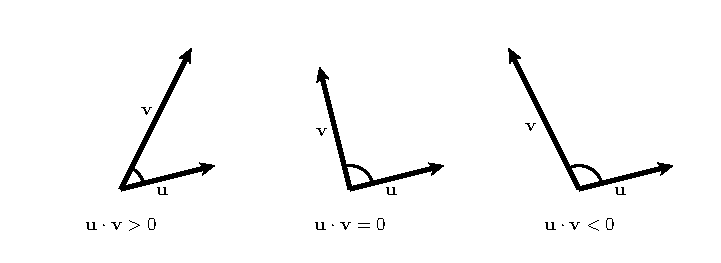
\includegraphics{figures/fig_9_3_orientations.eps}
    \caption{The orientation of vectors}
    \label{F:9.3.Orientations}
  \end{center}
\end{figure}

\newpage


\subsection*{Work, Force, and Displacement}

In physics, work is a measure of the energy required to apply a force
to an object through a displacement.  For instance, Figure
\ref{F:9.3.Work} shows a force $\vF$ displacing an object from point
$A$ to point $B$.  The displacement is then represented by the
vector $\overrightarrow{AB}$.  

\begin{figure}[ht]
  \begin{center}
    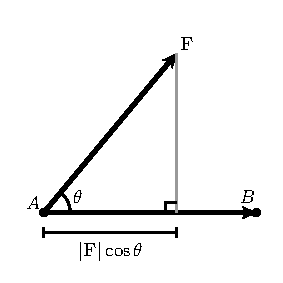
\includegraphics{figures/fig_9_3_work_1.eps}
  \end{center}
  \caption{A force $\vF$ displacing an object.}
  \label{F:9.3.Work}
\end{figure}

It turns out that the work required to displace the object is
$$
W = \vF\cdot\overrightarrow{AB} = |\vF||\overrightarrow{AB}|\cos\theta.
$$
This means that the work is determined only by the magnitude of the
force applied parallel to the displacement.  Consequently, if we are
given two vectors $\vu$ and $\vv$, we would like to write $\vu$ as a
sum of two vectors, one of which is parallel to $\vv$ and one of which
is orthogonal to $\vv$.  We take up this task after the next activity.

\begin{activity} \label{A:9.3.1}  Determine the work done by a 25 pound force acting at a $30^{\circ}$ angle to the direction of the object's motion, if the object is pulled 10 feet.  In addition, is more work or less work done if the angle to the direction of the object's motion is $60^\circ$?
\end{activity}
\begin{smallhint}
Use $W = |\vF| \cos(\theta) |\vv|$.
\end{smallhint}
\begin{bighint}
Identify $|\vF|$, $\theta$, and $|\vv|$ in $W = |\vF| \cos(\theta) |\vv|$ from the given information.
\end{bighint}
\begin{activitySolution}
If $\vF$ is our force, then $|\vF| = 25$ pounds. The angle at which the force is acting is $\theta = 30^{\circ}$, and the object is moved 10 feet, so the work done is  
\[|\vF| \cos(\theta) |\vv| = 25 \cos\left(30^{\circ}\right)(10) = 125 \sqrt{3} \text{ lb-ft} \approx 216.5 \text{ lb-ft}.\]
If we increase the angle to $60^{\circ}$, then the work done is
\[|\vF| \cos(\theta) |\vv| = 25 \cos\left(60^{\circ}\right)(10) = 125 \text{ lb-feet}.\]
So the work done if the force is applied at the higher angle is less, but about 91.5 lb-ft. This should be expected -- less of the force is applied to the direction of motion at the higher angle, resulting in less work done.  
\end{activitySolution}
\aftera


\subsection*{Projections}

\begin{figure}[ht]
  \begin{center}
    \begin{minipage}{3in}
      \begin{center}
        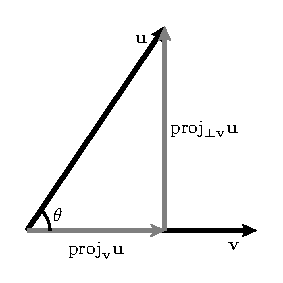
\includegraphics{figures/fig_9_3_projection_1.eps}
        \caption{The projection of $\vu$ onto $\vv$.}
        \label{F:9.3.Projection}
      \end{center}
    \end{minipage}
    \begin{minipage}{3in}
      \begin{center}
        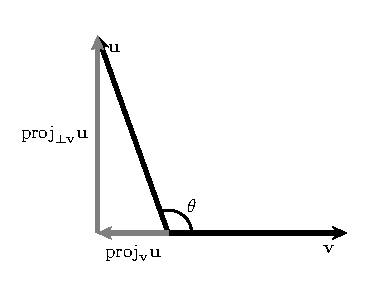
\includegraphics{figures/fig_9_3_projection_2.eps}
        \caption{$\proj_{\vv} \vu$ when $\theta > \frac\pi2$.}
        \label{F:9.3.Projection2}
      \end{center}
    \end{minipage}
  \end{center}
\end{figure}

Suppose we are given two vectors $\vu$ and $\vv$ as shown in Figure
\ref{F:9.3.Projection}.  Motivated by our discussion of work, we would
like to write $\vu$ as a sum of two vectors, one of which is parallel
to $\vv$ and one of which is orthogonal.  That is, we would like to
write 
\begin{equation}
  \vu = \proj_{\vv}\vu + \proj_{\perp\vv}\vu,
  \label{E:9.3.proj}
\end{equation}
where $\proj_{\vv}\vu$ is parallel to $\vv$ and $\proj_{\perp\vv}\vu$
is orthogonal to $\vv$.  
We call the vector $\proj_{\vv}\vu$ the
{\em projection} of $\vu$ onto $\vv$\index{vector!projection}.

To find the vector $\proj_{\vv} \vu$, we will dot both sides of Equation~(\ref{E:9.3.proj}) with the vector $\vv$, to find that
\begin{eqnarray*}
  \vu\cdot\vv& = &(\proj_{\vv}\vu + \proj_{\perp\vv}\vu)\cdot\vv \\
                   &=&(\proj_{\vv}\vu)\cdot\vv +
  (\proj_{\perp\vv}\vu)\cdot\vv \\
                  &=&(\proj_{\vv}\vu)\cdot\vv.\\
\end{eqnarray*}
Notice that $(\proj_{\perp\vv}\vu)\cdot\vv = 0$ since
$\proj_{\perp\vv}\vu$ is orthogonal to $\vv$.  Also, $\proj_{\vv}\vu$
must be a scalar multiple of $\vv$ since it is parallel to $\vv$, so we
will write $\proj_{\vv}\vu = s\vv$.  It follows that
$$
  \vu\cdot\vv =(\proj_{\vv}\vu)\cdot\vv = s\vv\cdot\vv,
$$
which means that
$$
s = \frac{\vu\cdot\vv}{\vv\cdot\vv}
$$
and hence
$$
\proj_{\vv}\vu = \frac{\vu\cdot\vv}{\vv\cdot\vv}\vv =
\frac{\vu\cdot\vv}{|\vv|^2}\vv 
$$

It is sometimes useful to write $\proj_{\vv}\vu$ as a scalar times a
unit vector in the direction of $\vv$.  We call this scalar the
{\em component of $\vu$ along $\vv$} and denote it as
$\comp_{\vv}\vu$.  We therefore have
$$
\proj_{\vv}\vu = \frac{\vu\cdot\vv}{|\vv|^2}\vv =
\frac{\vu\cdot\vv}{|\vv|} \frac{\vv}{|\vv|}=
\comp_{\vv}\vu \frac{\vv}{|\vv|},
$$
so that
$$
\comp_{\vv}\vu = \frac{\vu\cdot\vv}{|\vv|}.
$$

\vspace*{5pt}
\nin \framebox{\hspace*{3 pt}
  \parbox{6.25 in}{ Let $\vu$ and $\vv$ be vectors in $\R^n$. The
    component\index{vector!component in the direction of} of $\vu$ in
    the direction of $\vv$ is the scalar
    \[\comp_{\vv} \vu = \frac{\vu \cdot \vv}{|\vv|},\] and the
    projection\index{vector!projection} of $\vu$ onto $\vv$ is the
    vector \[\proj_{\vv} \vu = \frac{\vu \cdot \vv}{\vv\cdot\vv} \vv.\]
} \hspace*{3 pt}}
\vspace*{5pt}

Moreover, since
\[\vu = \proj_{\vv} \vu + \proj_{\perp \vv} \vu,\]
it follows that
\[\proj_{\perp \vv} \vu = \vu - \proj_{\vv} \vu.\]
This shows that once we have computed $\proj_{\vv} \vu$, we can find
$\proj_{\perp \vv} \vu$ simply by calculating the difference of two
known vectors.

\begin{activity} \label{A:9.3.4}  Let $\vu = \langle 2, 6 \rangle$ and $\vv = \langle 4, -8 \rangle$. Find $\comp_{\vv} \vu$, $\proj_{\vv} \vu$ and $\proj_{\perp \vv} \vu$, and draw a picture to illustrate.  Finally, express $\vu$ as the sum of two vectors where one is parallel to $\vv$ and the other is perpendicular to $\vv$.
\end{activity}
\begin{smallhint}
Use the projection formulas.
\end{smallhint}
\begin{bighint}
Recall that 
\begin{align*}
\comp_{\vv} \vu &= \frac{\vu \cdot \vv}{|\vv|} \\
\proj_{\vv} \vu &= \frac{\vu \cdot \vv}{|\vv|^2} \vv \\
\proj_{\perp \vv} \vu &= \vu - \proj_{\vv} \vu.
\end{align*}
\end{bighint}
\begin{activitySolution}
We know that 
\begin{align*}
\comp_{\vv} \vu &= \frac{\vu \cdot \vv}{|\vv|} = \frac{-40}{\sqrt{80}}, \\
\proj_{\vv} \vu &= \frac{\vu \cdot \vv}{|\vv|^2} \vv = -\frac{1}{2}\langle 4, -8 \rangle = \langle -2, 4 \rangle, \\
\proj_{\perp \vv} \vu &= \vu - \proj_{\vv} \vu = \langle 2, 6 \rangle - \langle -2, 4 \rangle = \langle 4,2\rangle.
\end{align*}
These vectors are illustrated below. 

%\begin{figure}[ht]
\begin{center}
\resizebox{!}{2.0in}{\includegraphics{figures/9_3_Act_4_sol}}
%\caption{Vectors and their projections.}
%\label{F:9.3.Act_4_sol}
\end{center}
%\end{figure}

\end{activitySolution}
\aftera


\begin{summary}
\item The dot product of two vectors in $\R^n$, $\vu = \langle u_1,
  u_2, \ldots, u_n \rangle$ and $\vv = \langle v_1, v_2, \ldots, v_n
  \rangle$, is the scalar
  \[
  \vu \cdot \vv = u_1v_1 + u_2v_2 + \cdots + u_nv_n.
  \]
\item The dot product is related to the length of a vector since
  $\vu\cdot\vu = |\vu|^2$.
\item The dot product provides us with information about the angle
  between the vectors since 
  \[
  \vu\cdot\vv = |\vu| \ |\vv|\cos\theta,
  \] 
  where $\theta$ is the angle
  between $\vu$ and $\vv$. 
\item Two vectors are orthogonal if the angle between them
  is $\pi/2$. In terms of the dot product, the vectors $\vu$ and
  $\vv$ are orthogonal if and only if $\vu \cdot \vv = 0$.
\item The projection of a vector $\vu$ in $\R^n$ onto a vector $\vv$
  in $\R^n$ is the vector
  \[
  \proj_{\vv} \vu = \frac{\vu \cdot \vv}{\vv\cdot\vv} \vv.
  \]
\end{summary}



\nin \hrulefill

\begin{exercises} 

\item \label{Ez:9.3.1}  Let $\vv = \langle -2, 5 \rangle$ in $\R^2$, and let $\vy = \langle 0, 3, -2 \rangle$ in $\R^3$. 

    \ba
    	\item Is $\langle 2, -1 \rangle$ perpendicular to $\vv$?  Why or why not?
	\item Find a unit vector $\vu$ in $\R^2$ such that $\vu$ is perpendicular to $\vv$.  How many such vectors are there?
	\item Is $\langle 2, -1, -2 \rangle$ perpendicular to $\vy$?  Why or why not?
	\item Find a unit vector $\vw$ in $\R^3$ such that $\vw$ is perpendicular to $\vy$.  How many such vectors are there?
	\item Let $\vz  = \langle 2, 1, 0 \rangle$.  Find a unit vector $\vr$ in $\R^3$ such that $\vr$ is perpendicular to both $\vy$ and $\vz$.  How many such vectors are there?
    \ea

\begin{exerciseSolution}

    \ba
    \item Since $\langle 2, -1 \rangle \cdot \langle -2, 5 \rangle = -9$ is not zero, the vector  $\langle 2, -1 \rangle$ is not perpendicular to $\vv$. 
	\item First we find a vector perpendicular to $\vv$. By inspection one such vector is $\vw=\langle 5, 2 \rangle$ (note that $\langle 5, 2 \rangle \cdot \vv = 0$). Then $\vu = \frac{1}{|\vw|} \vw = \frac{1}{\sqrt{29}} \langle 5,2 \rangle$ is a unit vector that is perpendicular to $\vv$.  There are exactly two unit vectors in $\R^2$ that are perpendicular to $\vv$: $\vu$ and $-\vu$. 
	\item The dot product of $\langle 2, -1, -2 \rangle$ with $\vy$ is 1, so these two vectors are not perpendicular. 
	\item The vector $\vy = \langle 0 , 2, 3 \rangle$ is perpendicular and so the vector $\vw = \frac{1}{|\vy|} \vy = \frac{1}{\sqrt{13}} \langle 0, 2, 3 \rangle$ is a unit vector in $\R^3$ that is perpendicular to $\vy$.  We can rotate the vector $\vw$ around the vector $\vv$ to obtain infinitely many different unit vectors in $\R^3$ that are perpendicular to $\vv$. 
	\item For a vector $\vr = \langle a,b,c \rangle$ to be perpendicular to both $\vy$ and $\vz$, we must have $\vr \cdot \vy = 0$ and $\vr \cdot \vz = 0$. This gives us two equations $3b-2c=0$ and $2a+b=0$. Thus, $b = -2a$ and $-6a-2c = 0$. So $c = -3a$. Thus, any vector of the form $\langle a, -2a, -3a \rangle$ is perpendicular to both $\vy$ and $\vz$. These vectors are all scalar multiples of the vector $\langle 1, -2, -3 \rangle$ with magnitude $\sqrt{14}$, and so there are just two vectors in $\R^3$ that are perpendicular to both $\vy$ and $\vz$: $\vr = \frac{1}{\sqrt{14}} \langle 1, -2, -3 \rangle$ and $-\vr$.   
    \ea
    
\end{exerciseSolution}

\item \label{Ez:9.3.2}  Consider the triangle in $\R^3$ given by $P(3, 2, -1)$, $Q(1, -2, 4)$, and $R(4, 4, 0)$.  
%Let $\va = \langle 2, -1, 1 \rangle$ and $\vb = \langle 1, 1, 3 \rangle$.

	\ba
		\item Find the measure of each of the three angles in the triangle, accurate to $0.01$ degrees.
		\item Choose two sides of the triangle, and call the vectors that form the sides (emanating from a common point) $\va$ and $\vb$.
			\begin{enumerate}[i.]
			\item Compute $\proj_{\vb} \va$, and $\proj_{\perp \vb} \va$.
			\item Explain why $\proj_{\perp \vb} \va$ can be considered a height of triangle $PQR$.
			\item Find the area of the given triangle.   
			\end{enumerate}
	\ea

\begin{exerciseSolution}

    \ba
    \item To find the angle between the sides $\overline{PQ}$ and $\overline{PR}$, we first we find the vectors that make up those sides of the triangle:  $\overrightarrow{PQ} = \langle -2, -4, 5 \rangle$, $\overrightarrow{PR} = \langle 1,2,1 \rangle$. Then the angle between $\overline{PQ}$ and $\overline{PR}$ is 
\[\cos^{-1}\left( \frac{\overrightarrow{PQ} \cdot \overrightarrow{PR}}{|\overrightarrow{PQ}| |\overrightarrow{PR}|} \right) = \cos^{-1}\left( \frac{-5}{\sqrt{45}\sqrt{6}}\right) \approx 107.72^{\circ}.\]
To find the angle between the sides $\overline{RQ}$ and $\overline{RP}$, we first we find the vectors that make up those sides of the triangle:  $\overrightarrow{RQ} = \langle -3, -6, 4 \rangle$, $\overrightarrow{RP} = \langle -1,-2,-1 \rangle$. Then the angle between $\overline{RQ}$ and $\overline{RP}$ is 
\[\cos^{-1}\left( \frac{\overrightarrow{RQ} \cdot \overrightarrow{RP}}{|\overrightarrow{RQ}| |\overrightarrow{RP}|} \right) = \cos^{-1}\left( \frac{11}{\sqrt{61}\sqrt{6}}\right) \approx 54.90^{\circ}.\]
To find the angle between the sides $\overline{QR}$ and $\overline{QP}$, we first we find the vectors that make up those sides of the triangle:  $\overrightarrow{QR} = \langle 3, 6, -4 \rangle$, $\overrightarrow{QP} = \langle 2,4,-5 \rangle$. Then the angle between $\overline{QR}$ and $\overline{QP}$ is 
\[\cos^{-1}\left( \frac{\overrightarrow{QR} \cdot \overrightarrow{QP}}{|\overrightarrow{QR}| |\overrightarrow{QP}|} \right) = \cos^{-1}\left( \frac{50}{\sqrt{61}\sqrt{45}}\right) \approx 17.38^{\circ}.\]
Note that  $107.72^{\circ} + 54.90^{\circ} + 17.38^{\circ} = 180^{\circ}$ as expected. 

	\item Choose two sides of the triangle, and call the vectors that form the sides (emanating from a common point) $\va$ and $\vb$.
		\begin{enumerate}[i.]
		\item Let $\va = \overrightarrow{PQ} = \langle -2, -4, 5 \rangle$ and $\vb = \overrightarrow{PR} = \langle 1,2,1 \rangle$. Then
\begin{align*}
\proj_{\vb} \va &= \frac{\va \cdot \vb}{\vb \cdot \vb} \vb = \frac{-5}{6} \langle 1,2,1 \rangle \\
\proj_{\va} \vb &= \frac{\vb \cdot \va}{\va \cdot \va} \va = \frac{-5}{45} \langle -2,-4,5 \rangle.
\end{align*}

		\item The vector $\proj_{\perp \vb} \va$ can be viewed as the vector from the tip of $\vb = \overrightarrow{PR}$ onto the line determined by the vector $\va$. This will be an altitude (or height) of the triangle. 
		\item The area of the triangle is one half the base times the height. We can use $\proj_{\perp \vb} \va$ as the height and $\va$ as teh base, so the area of the triangle is
\[\frac{1}{2} |\va| |\proj_{\perp \vb} \va| = \frac{1}{2} \sqrt{45} \left(\frac{5}{6}\right) \sqrt{6}.\]

	\end{enumerate}
    \ea
    
\end{exerciseSolution}

\item \label{Ez:9.3.3}    Let $\vu$ and $\vv$ be vectors in $\R^5$ with $\vu \cdot \vv = -1$, $| \vu | = 2$, $| \vv | = 3$, and $\theta$ the angle between $\vu$ and $\vv$. Use the properties of the dot product to find each of the following.
    \ba
    \item $\vu \cdot 2\vv$

    \item $(\vu + \vv) \cdot \vv$

    \item $(2\vu+4\vv) \cdot (\vu - 7\vv)$
    
    \item $\vv \cdot \vv$
    
    \item $|\vu| |\vv| \cos(\theta)$
    
    \item $\theta$

    \ea

\begin{exerciseSolution}
    \ba
    \item We know that we can factor scalars from dot products, so
\[\vu \cdot 2\vv = 2 (\vu \cdot \vv) = 2(-1) = -2.\]

    \item We know that $\vv \cdot \vv = |\vv|^2 = 9$.
    
    \item The dot product distributes over vector addition, so 
\[(\vu + \vv) \cdot \vv = (\vu \cdot \vv) + (\vv \cdot \vv) = (-1) + |\vv|^2 = (-1) + 9 = 8.\]

    \item Combing the distributive property of the dot product over vector addition, the fact that we can factor scalars from dot products, and that the dot product is commutative we see that  
\begin{align*}
(2\vu+4\vv) \cdot (\vu - 7\vv) &= 2(\vu \cdot \vu) - 14(\vu \cdot \vv) + 4(\vv \cdot \vu) - 28 (\vv \cdot \vv) \\
	&= 2(\vu \cdot \vu) - 14(\vu \cdot \vv) + 4(\vu \cdot \vv) - 28 (\vv \cdot \vv) \\
    &= 2(\vu \cdot \vu) - 10(\vu \cdot \vv) + 4(\vu \cdot \vv) \\
    &= 2|\vu|^2 - 10(\vu \cdot \vv) - 28 |\vv|^2 \\
    &= 8+10-252 \\
    &=-234.
 \end{align*}
 
    
    \item Given that $\cos(\theta) = \frac{\vu \cdot \vv}{|\vu| |\vv|}$, we have 
\[|\vu| |\vv| \cos(\theta) = \vu \cdot \vv = -1.\]
    
    \item In this case we have 
\[\theta = \cos^{-1}\left(\frac{\vu \cdot \vv}{|\vu| |\vv|}\right) = \cos^{-1}\left(\frac{-1}{6}\right) \approx 99.59^{\circ}.\] 

    \ea
    
\end{exerciseSolution}



%\item \label{Ez:9.3.1}   

%A tetrahedron is a four-sided solid in $\R^3$, each of whose faces are triangles.  Consider the tetrahedron whose vertices are the points $(1,0,0)$, $(0,1,0)$, $(1,0,0)$, and $(1,1,1)$ as shown in Figure
%\begin{figure}[ht]
%\begin{center}
 %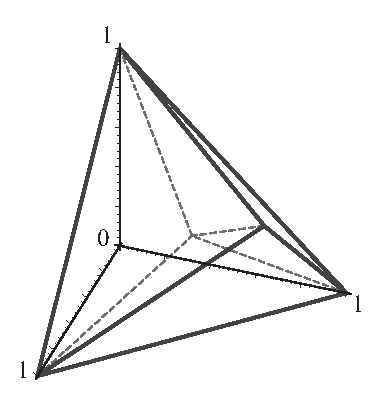
\includegraphics{figures/9_3_Ez1_tetrahedron.eps}
% \caption{The tetrahedron with vertices $(1,0,0)$, $(0,1,0)$, $(1,0,0)$, and $(1,1,1)$.} \label{F:9_3_Ez1_tetrahedron}
%\end{center}
%\end{figure}
%The \emph{centroid} of the tetrahedron is the average of the four vertices, which is the point $(\frac{1}{2}, \frac{1}{2}, \frac{1}{2})$, as shown at the intersection of the dotted lines.
 %   \ba
  %  	\item Consider the face determined by $(1,0,0)$, $(1,1,1)$, and $(0,0,1)$.  Explain why this face is an equilateral triangle.
%	\item 
 %   \ea

%\begin{exerciseSolution}
%\end{exerciseSolution}

\end{exercises}
\afterexercises


\clearpage
